% Files using this must be two subfolders
% deep. Adjust the number of ../ for the
% depth of the file.
% Imports
\usepackage{fancyhdr}
\usepackage{geometry}
\usepackage{icomma}
\usepackage{amsmath}
\usepackage{multicol}
\usepackage{mathptmx}
\usepackage{anyfontsize}
\usepackage{t1enc}
\usepackage{tabto}
\usepackage{listings}
\usepackage{filecontents}
\usepackage{subcaption}
\usepackage{tikz}
\usepackage[parfill]{parskip}
\usepackage{graphicx}
\usepackage[]{mdframed}
\usepackage{amsmath}
\usepackage[makeroom]{cancel}
\usepackage{pgfplots}
\usepackage{pgfplotstable}
\usepackage{xfrac}
\usepackage{amssymb}
\usepackage{mathtools}
\pgfplotsset{compat=1.18}
\usetikzlibrary{patterns}
\usepgfplotslibrary{polar}
\usepgfplotslibrary{fillbetween}

\geometry{margin=2.5cm}

\newcommand{\name}{Kaleb Burris}
\newcommand{\classname}{MATH F253, Elizabeth S. Allman, University of Alaska Fairbanks}
\newcommand{\assignment}{FILL IN ASSIGNMENT NAME}

\pagestyle{fancy}

\fancyhead[L]{
    \name 
    \newline
    \classname
    \newline
    \assignment
}

\newcommand{\horizontal}{\noindent\rule{\hsize}{0.4pt}}

\setlength{\headheight}{42pt}
\setlength{\headsep}{0.25in}
\setlength{\columnsep}{0.35cm}
\setlength{\columnseprule}{1pt}

\usepackage[T1]{fontenc}
\usepackage{lmodern}

\usepackage{graphicx}
\graphicspath{ {./lab0images/} }

% Put class number, class name, and professor 
% name.
% Use only in case of emergency, this
% should be covered by the preamble.
% \renewcommand\classname{}

% Put the assignment name with \S if 
% necessary for the section and the question 
% numbers.
\renewcommand\assignment{HW 1, Due Friday, 1/27/2023 23:59; \#19,28,35,40,43,47}

\begin{document}

    % Templates
    \iffalse
    % Use these for equations.
    \begin{equation*}
        \begin{gathered}
            Equations go here.
        \end{gathered}
    \end{equation*}

    % Use this if a line of math is too long.
    \resizebox{\hsize}{!}{$Long equation goes here$}

    % Use these for multiple columns.
    \begin{multicol*}{# of columns}
        % Remove the * if you want the columns to be balanced.
    \end{multicol*}

    % Use this to add a horizontal line.
    \horizontal

    \fi

    % Begin homework here.
    %%%%%%%%%%%%%%%%%%%%%%

    \begin{multicols*}{2}
        \paragraph*{19.}
        Write a short description of the motion of a real object for which FIGURE EX.1.19 would be a realistic position-versus-time graph.

        \begin{mdframed}
            An elevator brings its occupants up 100 meters before stopping to let them off. It then shoots up another 200 meters to the top story of the building.
        \end{mdframed}

        \paragraph*{28.}
        Compute the following numbers, applying the significant figure rules adopted in this textbook.

        \begin{mdframed}
            a. $33.3 \times 25.4 = \boxed{846}$

            b. $33.3 - 25.4 = \boxed{28.9}$

            c. $\sqrt(33.3) = \boxed{5.77}$

            d. $333.3 \div 25.4 = \boxed{13.1}$
        \end{mdframed}

        \paragraph*{35.}
        A jetplane is cruising at 300 m/s when suddenly the pilot turns the engines up to full throttle. After traveling 4.0 km, the jet is moving with a speed of 400 m/s. What is the jet's acceleration as it speeds up?

        \begin{mdframed}
            \begin{equation*}
                \begin{gathered}
                    \vec{a} = \frac{\Delta v}{\Delta t} = \frac{100}{\Delta t}  \\
                    \Delta t = \frac{\Delta s}{\vec{\overline{v}}} = \frac{4000}{350} = 11.4    \\
                    \vec{a} = \frac{100}{11.4} = \boxed{8.77 \text{m/s}^2}
                \end{gathered}
            \end{equation*}
        \end{mdframed}

        \paragraph*{40.}
        A motorist is traveling at 20 m/s. He is 60 m from a stoplight when he sees it turn yellow. His reaction time, before stepping on the brake, is 0.50 s. What steady deceleration while braking will bring him to a stop right at the light?

        \begin{mdframed}
            \begin{equation*}
                \begin{gathered}
                    d_{sl} = 60 - 20(0.5) = 50 m \quad \vec{v}_0 = 20 \text{m/s}    \\
                    \vec{a} = \frac{\Delta v}{\Delta t} = \frac{-20}{\Delta t}      \\
                    \Delta t = \frac{d_{sl}}{\overline{\vec{s}}} = \frac{50}{10} = 5 \\
                    \vec{a} = -\frac{20}{4} = boxed{-4\text{m/s}^2}
                \end{gathered}
            \end{equation*}
        \end{mdframed}

        \paragraph*{43.}

        \begin{mdframed}
            \begin{tikzpicture}
                \begin{axis}[    axis lines=middle,    xmin=-5,xmax=5,    ymin=-5,ymax=5,    xtick={-5,...,5},    ytick={-5,...,5},    xlabel=$x$,    ylabel=$y$,    clip=false,    ]
                    \addplot[fill=blue!20,draw=blue!50!black] coordinates {(-4,-4) (-4,4) (4,4) (4,-4)};
                    \addplot[fill=green!20,draw=green!50!black] coordinates {(-3,-3) (-3,3) (3,3) (3,-3)};
                    \addplot[fill=red!20,draw=red!50!black] coordinates {(-2,-2) (-2,2) (2,2) (2,-2)};
                    \addplot[fill=yellow!20,draw=yellow!50!black] coordinates {(-1,-1) (-1,1) (1,1) (1,-1)};
                \end{axis}
                \end{tikzpicture}
        \end{mdframed}
        

    \end{multicols*}
\end{document}